\begin{enumerate}[label=\thesubsection.\arabic*.,ref=\thesubsection.\theenumi]
\numberwithin{equation}{enumi}

\item Generate the Routh array for the 
polynomial, 
\begin{align}
f(s)=s^{7}+s^{6}+7 s^{5}+14 s^{4}+31s^{3}+73 s^{2}+25 s+ 200
\label{eq:ee18btech11014_routh_poly}
\end{align}
\solution 
\begin{align}
\mydet{s^7\\s^6\\s^5}
\mydet{1 & 7 & 31 & 25 \\ 1 & 14 & 73 & 200 \\ -7 & -42 & -175 & 0}
\end{align}\\
\begin{align}
\mydet{s^7\\s^6\\s^5\\s^4}
\mydet{1 & 7 & 31 & 25 \\ 1 & 14 & 73 & 200 \\ -7 & -42 & -175 & 0 \\ 8 & 48 & 200 & 0}
\end{align}\\
\begin{align}
\mydet{s^7\\s^6\\s^5\\s^4\\s^3}
\mydet{1 & 7 & 31 & 25 \\ 1 & 14 & 73 & 200 \\ -7 & -42 & -175 & 0 \\ 8 & 48 & 200 & 0 \\ 0 & 0 & 0 &  }
\end{align}\\

When such a case is encountered, we take the derivative of the expression formed the the coefficients above it i.e derivative of $8s^4 + 48s^2 +200$.
\begin{center}
    $\frac{d}{dx}(8s^4 + 48s^2 +200) = 32s^3 + 96s$
\end{center}

The coefficients of obtained expression are placed in the table.

\begin{align}
\mydet{s^7\\s^6\\s^5\\s^4\\s^3}
\mydet{1 & 7 & 31 & 25 \\ 1 & 14 & 73 & 200 \\ -7 & -42 & -175 & 0 \\ 8 & 48 & 200 & 0 \\ 32 & 96 & 0 &  }
\end{align}\\
\begin{align}
\mydet{s^7\\s^6\\s^5\\s^4\\s^3\\s^2}
\mydet{1 & 7 & 31 & 25 \\ 1 & 14 & 73 & 200 \\ -7 & -42 & -175 & 0 \\ 8 & 48 & 200 & 0 \\ 32 & 96 & 0 &  \\ 24 & 200 & 0 &  }
\end{align}\\
\begin{align}
\mydet{s^7\\s^6\\s^5\\s^4\\s^3\\s^2\\s^1}
\mydet{1 & 7 & 31 & 25 \\ 1 & 14 & 73 & 200 \\ -7 & -42 & -175 & 0 \\ 8 & 48 & 200 & 0 \\ 32 & 96 & 0 &  \\ 24 & 200 & 0 &  \\ -170.67 & 0 &  & }
\end{align}\\
\begin{align}
\mydet{s^7\\s^6\\s^5\\s^4\\s^3\\s^2\\s^1\\s^0}
\mydet{1 & 7 & 31 & 25 \\ 1 & 14 & 73 & 200 \\ -7 & -42 & -175 & 0 \\ 8 & 48 & 200 & 0 \\ 32 & 96 & 0 &  \\ 24 & 200 & 0 &  \\ -170.67 & 0 &  & \\200 &   &   & }
\label{eq:ee18btech11014_routh_final}
\end{align}

So, the above one is the Routh-Hurwitz Table.

\item Find the number of roots of the polynomial in the right half of the $s$-plane.
\\
\solution The number of roots of the polynomial that are in the right half-plane is equal to
the number of sign changes in the first column. From \ref{eq:ee18btech11014_routh_final},
the polynomial in \eqref{eq:ee18btech11014_routh_poly}
has 4 roots lie on right-side of Imaginary Axis.

\item Write a Python code for generating each stage of the Routh Table.
\\
\solution The following code 
\begin{lstlisting}
codes/ee18btech11014/Routh_Hurwitz_Stages.py
\end{lstlisting}
%
generates the various stages.
%The below image is the location of Roots of given polynomial.\\
%%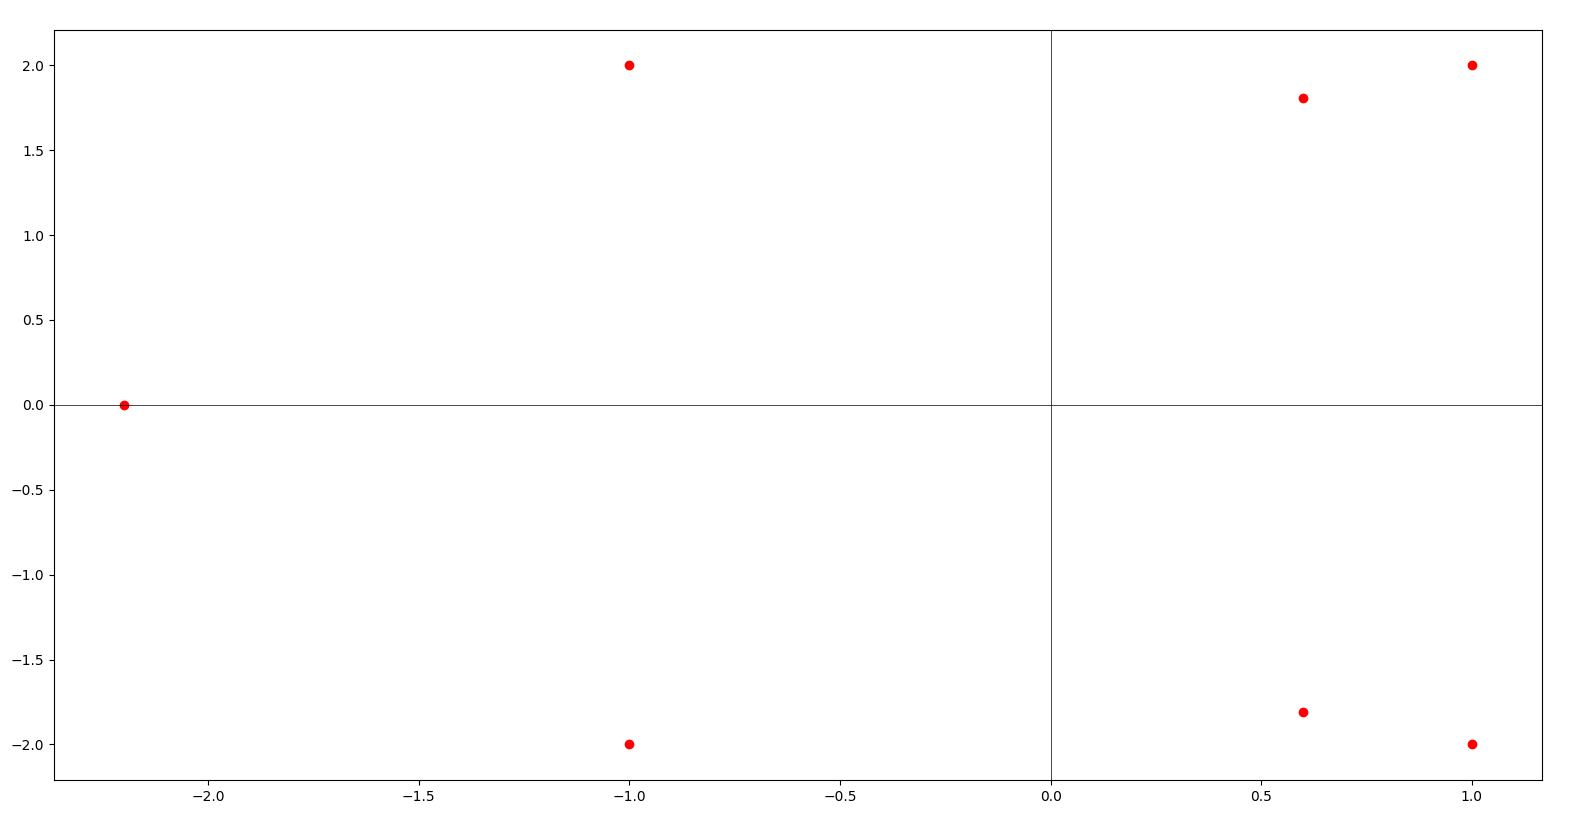
\includegraphics[scale=0.15]{figs/Roots.eps}\\
%
%The below image is finding out the roots of given polynomial by substituting $z=x+iy$ and obtaining the Real and Imaginary Parts of f(z). The values of $z$ where Real and Imaginary parts f(z) becomes zero simultaneously are roots of f(z).\\
%%\includegraphics[scale=0.15]{figs/f(z).png}

\item Find the roots of the polynomial in in \eqref{eq:ee18btech11014_routh_poly} and verify that 4 roots are in the right half $s$-plane.
\\
\solution The following code generates the necessary roots.
\begin{lstlisting}
codes/ee18btech11014/Roots.py
\end{lstlisting}
\end{enumerate}
